%%%%%%%%%%%%%%%%%%%%%%%%%%%%%%%%%%%%%%%%%%%%%%%%%%%%%%%%%%%%%%%%%%%%%%%%%%%%%%%%%%
\begin{frame}[fragile]\frametitle{}
\begin{center}
{\Large Neo4j}
\end{center}
\end{frame}


%%%%%%%%%%%%%%%%%%%%%%%%%%%%%%%%%%%%%%%%%%%%%%%%%%%%%%%%%%%
\begin{frame}[fragile]\frametitle{Introduction}

\begin{itemize}
\item 
\end{itemize}

\end{frame}


%%%%%%%%%%%%%%%%%%%%%%%%%%%%%%%%%%%%%%%%%%%%%%%%%%%%%%%%%%%
\begin{frame}[fragile]\frametitle{Windows Installation}

\begin{itemize}
\item Have Open JDK 11 ready, if not, go to https://learn.microsoft.com/en-us/java/openjdk/download (178 MB)
\item https://neo4j.com/download-center/\#community (4.4.11 129 MB)
\item Place the extracted files in a permanent home on your server, for example \lstinline|D:\neo4j\|. The top level directory is referred to as NEO4J\_HOME.
\item To run Neo4j as a console application, use: \lstinline|<NEO4J_HOME>\bin\neo4j console|

\begin{lstlisting}
C:\neo4j\bin>neo4j.bat console
Directories in use:
home:         C:\neo4j
:
Starting Neo4j.
\end{lstlisting}

\item Visit http://localhost:7474 in your web browser.
\item Default login is username 'neo4j' and password 'neo4j' Change password. Got conncted to `neo4j://127.0.0.1:7687`
\end{itemize}

\end{frame}


%%%%%%%%%%%%%%%%%%%%%%%%%%%%%%%%%%%%%%%%%%%%%%%%%%%%%%%%%%%
\begin{frame}[fragile]\frametitle{Console}

\begin{center}
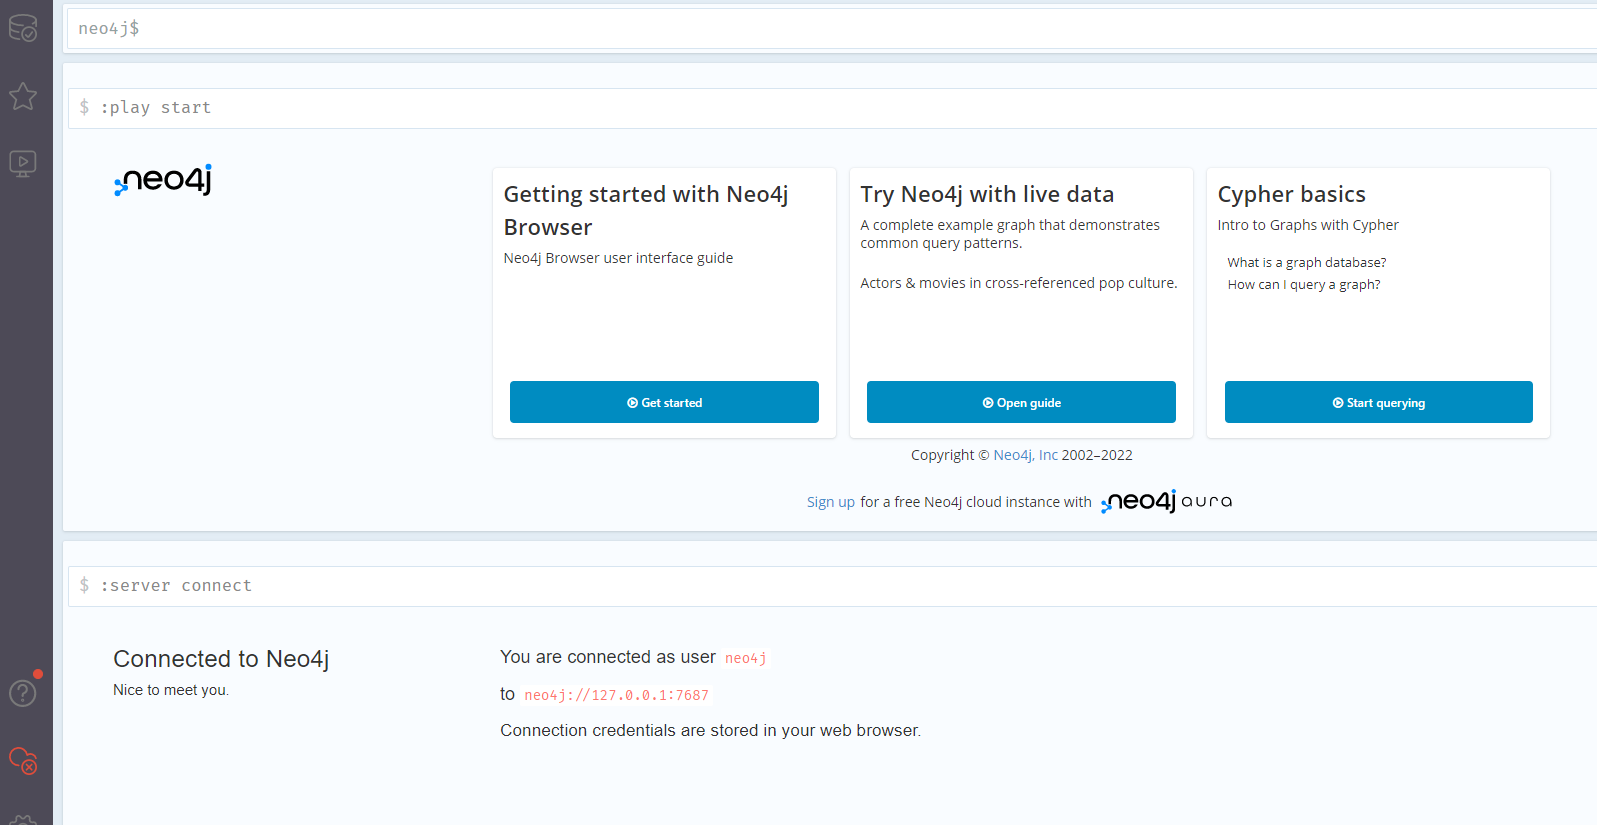
\includegraphics[width=\linewidth,keepaspectratio]{neo4j1}
\end{center}	  

\end{frame}

%%%%%%%%%%%%%%%%%%%%%%%%%%%%%%%%%%%%%%%%%%%%%%%%%%%%%%%%%%%
\begin{frame}[fragile]\frametitle{Interaction}

Type commands in top command window

\begin{itemize}
\item \lstinline|MATCH(n) RETURN n| Return nodes (type none). As there is nothing, nothing gets returned. So create something.
\item \lstinline|CREATE(n)| will create one empty node.
\item \lstinline|MATCH(n) RETURN n| will now return 1 node and show it.
\end{itemize}

\begin{center}
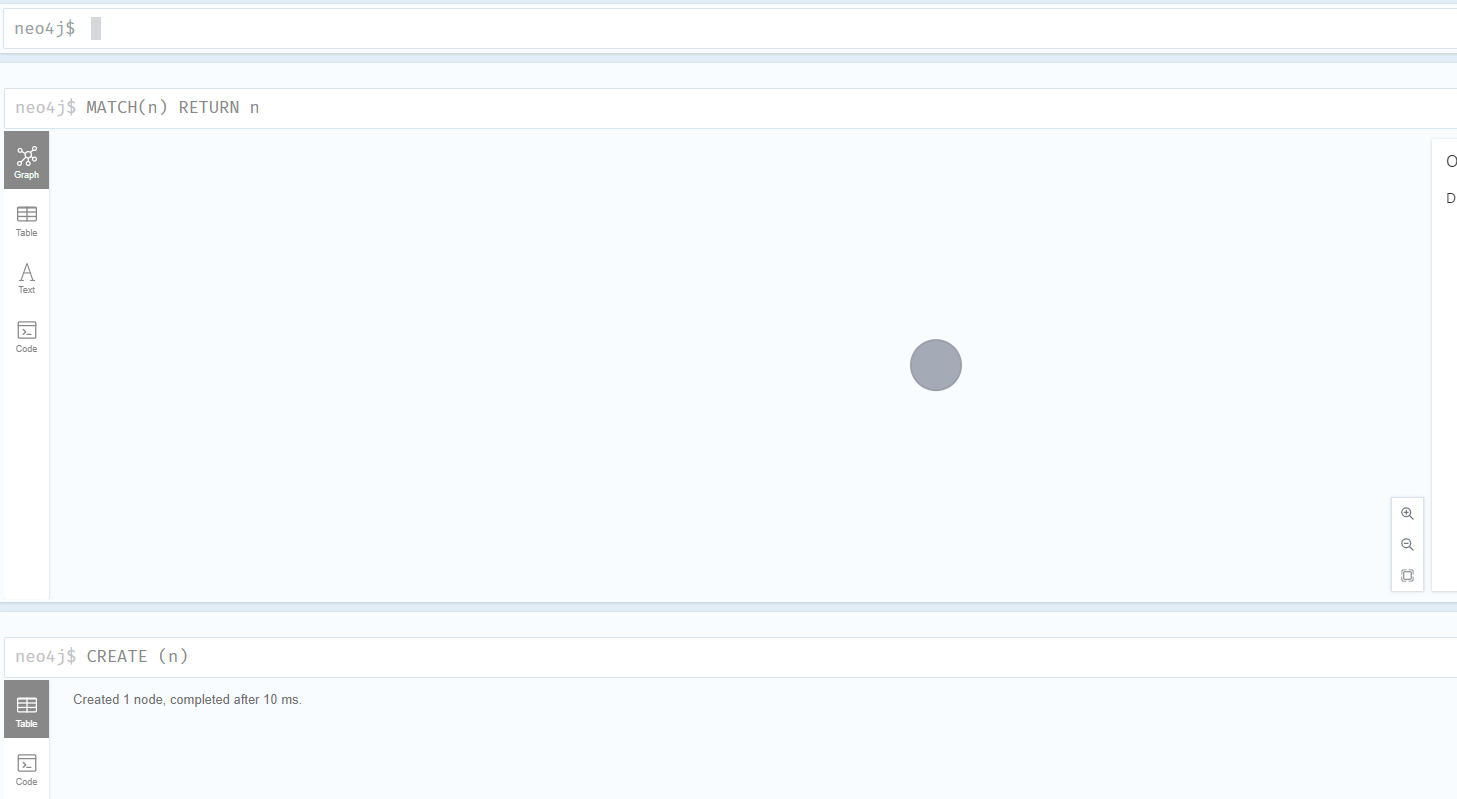
\includegraphics[width=0.8\linewidth,keepaspectratio]{neo4j2}
\end{center}

\end{frame}


%%%%%%%%%%%%%%%%%%%%%%%%%%%%%%%%%%%%%%%%%%%%%%%%%%%%%%%%%%%
\begin{frame}[fragile]\frametitle{Examples}

\begin{itemize}
\item \lstinline|CREATE(n:PERSON)| create a node (type PERSON). Type is actually the label of the node.
\item \lstinline|MATCH(n) DELETE(n)| will delete all the nodes
\item \lstinline|CREATE(n:PERSON{name:'chris', favoritecolor:'blue'})| create a node (type PERSON) along with some properties. SImilariy, can create different nodes of different type.
\item \lstinline|MATCH(n:PERSON) RETURN (n)|to selectively return only PERSONs.
\item \lstinline|MATCH(n) RETURN (n) LIMIT 4| to return only 4 nodes
\item Two create relationship find 2 nodes using \lstinline|MATCH| and \lstinline|WHERE| to restrict, then create relationship 'studied\_at'

\begin{lstlisting}
MATCH (s:School), (p:Person)
WHERE s.name = 'LSU' and p.name = 'jenny'
CREATE (p)-[stu:STUDIED_AT]->(s)
\end{lstlisting}


\end{itemize}

\end{frame}


%%%%%%%%%%%%%%%%%%%%%%%%%%%%%%%%%%%%%%%%%%%%%%%%%%%%%%%%%%%
\begin{frame}[fragile]\frametitle{Examples}


\begin{center}
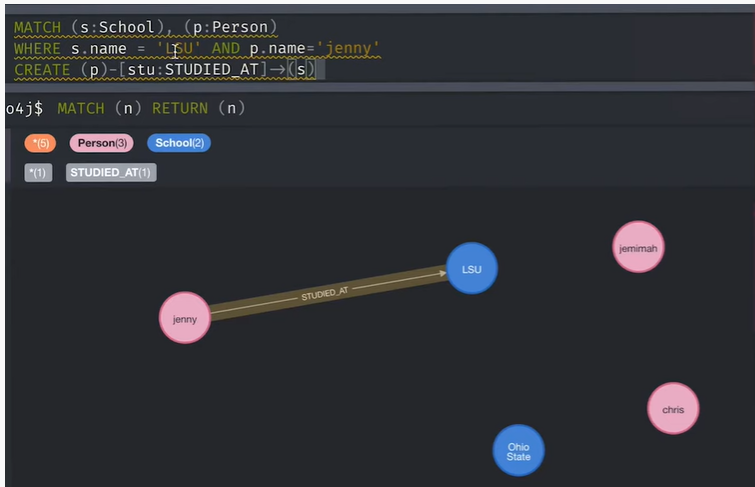
\includegraphics[width=0.9\linewidth,keepaspectratio]{neo4j3}
\end{center}	

{\tiny (Ref: An introduction to neo4j (graph database tutorial for beginners) - Chris Hay)}

\end{frame}


